%%%%%%%%%%%%%%%% Springer LNCS paper %%%%%%%%%%%%%%%%%%%%%%%%%%%%%%%

\documentclass[runningheads]{llncs}

\usepackage[T1]{fontenc}
\usepackage{amsmath}
\usepackage{amssymb}
\usepackage{booktabs}
\usepackage{graphicx}
\usepackage{listings}
\usepackage{xcolor}
\usepackage{tikz}
\usepackage{array}
\usepackage{multirow}
\usepackage{url}
\usepackage{microtype}
\usepackage{etoolbox}
\usepackage{mathpartir}
\usepackage{placeins}
\usetikzlibrary{arrows.meta,positioning,shapes.geometric}
\setlength{\textfloatsep}{8pt plus 2pt minus 2pt}
\setlength{\floatsep}{8pt plus 2pt minus 2pt}
\setlength{\intextsep}{8pt plus 2pt minus 2pt}
\emergencystretch=2em

\lstdefinelanguage{Coq}{
  morekeywords={Inductive,Type,forall,Theorem,true,false,inr},
  sensitive=true,
  morecomment=[s]{(*}{*)}
}

\lstset{
  basicstyle=\ttfamily\footnotesize,
  keywordstyle=\color{blue!60!black},
  commentstyle=\color{gray!70!black},
  numbers=left,
  numberstyle=\tiny\color{gray},
  numbersep=5pt,
  breaklines=true,
  frame=single,
  tabsize=2,
  captionpos=b,
  aboveskip=0.4em,
  belowskip=0.4em
}

\newcommand{\encore}{\textit{Encore!}}
\newcommand{\rocq}{Rocq}
\newcommand{\code}[1]{\texttt{#1}}
\newcommand{\derive}[1]{\texttt{\#\allowbreak[derive(#1)]}}

\begin{document}

\title{From Rocq to Metal: A Pipeline for Formally Verified Microcontroller Firmware}
\titlerunning{From Rocq to Metal}

\author{Valentin Bergeron\inst{1} \and Karolina Gorna\inst{2}}
\authorrunning{V. Bergeron and K. Gorna}
\institute{
Ledger, Paris, France\\
\email{valentin.bergeron@ledger.fr}
\and
Telecom Paris and Ledger Donjon, Paris, France\\
\email{karolina.gorna@[telecom-paris,ledger].fr}
}

\maketitle

\begin{abstract}
Enforcing invariants in safety-critical firmware is increasingly urgent as generated code becomes widespread, but standard extraction targets for proof assistants require runtimes too large for many embedded devices.
We present a pipeline for running formally verified Rocq firmware logic on Cortex-M microcontrollers.
The pipeline extracts Gallina to Scheme, compiles it with \encore, a bare-metal Continuation Passing Style (CPS) bytecode virtual machine, and embeds the result in \code{no\_std} Rust firmware.
We structure applications as pure state-transition functions, so the business logic is proved in Rocq while the event/effect boundary, host callbacks, compiler, and VM remain explicit trusted components: no proof yet relates bytecode execution to Gallina semantics.
On ST33-class targets with a 50 KB RAM lower bound, \encore{} executes unmodified Rocq-extracted code, stays within the target memory budget on our benchmarks, and validates a transaction-signing application on physical Ledger Flex hardware.

\keywords{formal verification \and Rocq \and Gallina \and microcontrollers \and firmware \and CPS \and proof extraction}
\end{abstract}

\section{Introduction}

Generated code is changing how software is written, including firmware.
For safety-critical devices, lower code-generation cost increases the amount of code that must be reviewed, while the required assurance level remains high.
Formal verification has already demonstrated its value at the systems level (seL4~\cite{klein2009sel4} gives a machine-checked proof of OS kernel correctness), and similar rigour is increasingly sought for firmware.
Formal specifications offer a scalable response: generated implementations can be checked against theorem statements, and proof obligations become part of the development interface.

However, the hardware constraints of embedded firmware prevent straightforward use of standard specification language extraction.
The runtimes required to execute extracted code exceed the resource budget of most microcontrollers.
Standard practice is therefore to translate specifications into the host language, automate that translation, or use host-language extensions, weakening the connection to the proof assistant.

We built \encore{}~\cite{encore} to close this gap.
\encore{} is a bare-metal CPS bytecode VM written in \code{no\_std} Rust that executes Rocq-extracted Scheme on microcontrollers.
The pipeline covers the whole path from proof to device: write firmware logic and prove it correct in Rocq, extract to Scheme, compile with \encore, and deploy.
What runs on the MCU is directly derived from the Rocq source, though the compiler, VM, host callbacks, and device I/O remain trusted.

We first present an architecture for structuring firmware so its core is fully verifiable, illustrated on a concrete transaction-signing application.
Next, we introduce \encore{}, the runtime we built to execute this code on microcontrollers.
We then survey the existing extraction paths from theorem provers to embedded targets, and characterize why they fall short on this class of hardware.
Finally, we present experimental results and outline remaining steps toward extending trust further up the toolchain.

This work makes three contributions:
\begin{itemize}
  \item We show that code extracted from Rocq can run on Cortex-M microcontrollers, by choosing Scheme as the extraction target and building a purpose-built bare-metal runtime.
  \item We present \encore, a \code{no\_std} CPS bytecode VM in Rust that fits within the resource budget of ST33-class hardware and executes unmodified Rocq-extracted Scheme.
  \item We introduce a firmware architecture structured as a pure state-transition function, making the business-logic core fully provable in Rocq while confining the unverified trusted computing base (TCB) to the event/effect boundary, which grows with the hardware interface rather than with application logic.
\end{itemize}

\section{An Architecture for Verified Firmware}
\label{sec:firmware}

This section answers \emph{what} to run on the MCU and how to structure it so correctness is fully provable in Rocq.

\subsection{The State Transition Model}

The model below is not imported from an existing specification: we define it for this work.
Its shape follows the well-established reactive state-machine pattern (an application reduced to a transition over an explicit state driven by input events), which we instantiate for firmware.
We choose this formulation because it maximizes the area that can be proven: modelling the application as a pure state transition function, effectively treating the whole embedded device as a state machine, confines all impurity to the event and effect boundary and leaves the transition itself as pure Gallina we can reason about directly.

Before diving into the modeling details, we assume that a Scheme VM is deployed as part of what we call a Formal Software Development Kit (FSDK), that bridges the virtual machine and the host device.
The FSDK contains both host code (it \emph{is} the real firmware that gets deployed) and Rocq code to provide the necessary bridge abstractions.

With this in mind, we define the state transition function as:
\[
  \code{step} : \code{State} \times \code{Event} \rightarrow \code{State} \times \code{list}\ \code{Effect}.
\]

Given the types:
\begin{description}
  \item[\textbf{State}] represents the application state. This will depend on what problem the application is solving, independently from the FSDK.
  \item[\textbf{Event}] is an incoming event from the device. Device events are linked to the underlying hardware and can be network packets, user interface signals such as pressed buttons or specific touch screen positions, etc.
  \item[\textbf{Effect}] is the description of an effectful computation that needs to be interpreted to be realized. A critical part of the FSDK is then to interpret the effects to perform them.
\end{description}

This model applies two key functional programming principles, copying instead of mutating and describing effects rather than performing them directly, to firmware code, effectively maximizing the provable business logic part.

The remaining parts, the \textbf{Event poller} and the \textbf{Effect interpreter}, form the TCB.
Their size is independent of firmware complexity unless new hardware operations and capabilities are added.
The verified core grows with the application; the unverified boundary grows only with the hardware interface.

Moreover, in a VM-based deployment the application logic can be fully specified in the VM input code, allowing the same carefully reviewed base firmware to host custom, verified business logic, which is a particularly powerful combination for safety-critical devices.

\subsection{Admitted Axioms and the Trust Chain}
\label{sec:axioms}

Some operations are observationally pure from Rocq's perspective but will be extremely impractical to implement fully from a business point of view.
For instance, hash functions, polynomial operations (CRC), and more generally any finite field operation involved in cryptographic algorithms.

Rather than relying on an Effect/Event pair with little added value, we choose to admit them in Rocq as axioms and provide them as host callbacks before the application run loop starts.
Additionally, VM primitive operations such as raw byte operations (\code{bytes\_len}, \code{bytes\_concat}, etc.) are abstracted via a typeclass admitted in the extraction context.
The FSDK bridges the typeclass and the concrete VM-provided implementations via Rocq extraction directives.

This bridge is currently manual, not automated: each host primitive is declared once in Rocq as an axiom giving its type, its intended behavior is stated as an accompanying Rocq axiom when a proof depends on it, and an extraction directive links the name to the Rust callback.
Adding or changing a primitive on the Rust host therefore requires a matching Rocq-side edit; there is no tool that infers Rocq signatures or specifications from the host code.
This keeps the trusted axioms few and auditable, at the cost of manual upkeep, and automating this correspondence is left as future work.

\begin{figure}
\centering
\resizebox{\textwidth}{!}{%
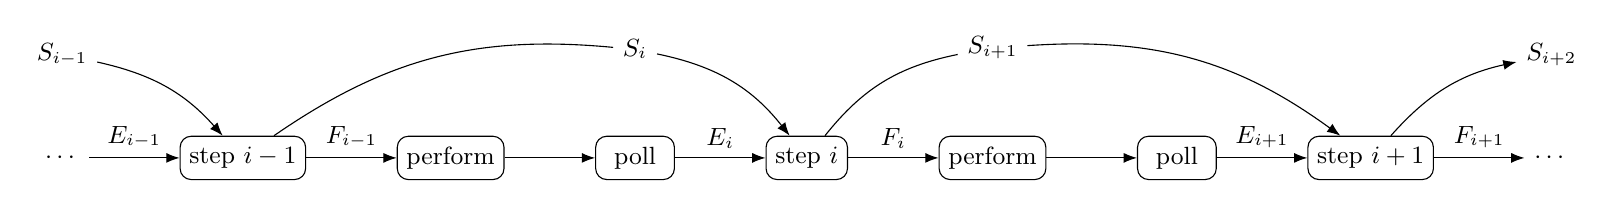
\begin{tikzpicture}[
  node distance=1.15cm,
  every node/.style={font=\small},
  stepnode/.style={draw, rounded corners, minimum width=1.0cm, minimum height=0.55cm},
  arr/.style={-Latex}
]
  \node (dotsl) {$\cdots$};
  \node[stepnode, right=of dotsl] (stepa) {step $i-1$};
  \node[stepnode, right=of stepa] (perfa) {perform};
  \node[stepnode, right=of perfa] (polla) {poll};
  \node[stepnode, right=of polla] (stepb) {step $i$};
  \node[stepnode, right=of stepb] (perfb) {perform};
  \node[stepnode, right=of perfb] (pollb) {poll};
  \node[stepnode, right=of pollb] (stepc) {step $i+1$};
  \node[right=of stepc] (dotsr) {$\cdots$};

  \draw[arr] (dotsl) -- node[above] {$E_{i-1}$} (stepa);
  \draw[arr] (stepa) -- node[above] {$F_{i-1}$} (perfa);
  \draw[arr] (perfa) -- (polla);
  \draw[arr] (polla) -- node[above] {$E_i$} (stepb);
  \draw[arr] (stepb) -- node[above] {$F_i$} (perfb);
  \draw[arr] (perfb) -- (pollb);
  \draw[arr] (pollb) -- node[above] {$E_{i+1}$} (stepc);
  \draw[arr] (stepc) -- node[above] {$F_{i+1}$} (dotsr);

  \node[above=0.85cm of dotsl] (sim1) {$S_{i-1}$};
  \node[above=0.85cm of polla] (si) {$S_i$};
  \node[above=0.85cm of perfb] (sip1) {$S_{i+1}$};
  \node[above=0.85cm of dotsr] (sip2) {$S_{i+2}$};
  \draw[arr] (sim1) to[bend left=18] (stepa);
  \draw[-] (stepa) to[bend left=20] (si);
  \draw[arr] (si) to[bend left=20] (stepb);
  \draw[-] (stepb) to[bend left=20] (sip1);
  \draw[arr] (sip1) to[bend left=20] (stepc);
  \draw[arr] (stepc) to[bend left=18] (sip2);
\end{tikzpicture}
}
\caption{Formal SDK generic app loop over two consecutive steps. $S$: State, $E$: Event, $F$: Effects list. Ellipses denote the unbounded continuation of the loop.}
\label{fig:funloop}
\end{figure}

\subsection{Trust Assumptions}
\label{sec:trust}

The verified part of the system is the Rocq model of the application logic and its stated properties.
The trusted computing base includes the Rocq kernel and extraction mechanism, the extracted Scheme frontend, the \encore{} compiler and VM, the Rust compiler, host callbacks implementing admitted axioms, and the event poller/effect interpreter supplied by the device firmware.
This boundary is deliberate: application growth extends the proved \code{step} function and its lemmas, whereas the unverified boundary changes only when new hardware actions, externs, or runtime primitives are added.
The current work therefore establishes verified firmware logic running on bare metal; Sect.~\ref{sec:semantics} states the compiler correctness theorem that would remove the compiler and VM from this list, and proving it is future work, discussed in Sect.~\ref{sec:discussion}.

\subsection{Concrete Example: Transaction Signing Application}

As a concrete example, we built a Ledger Flex transaction-signing app with \encore.

LedgerOS provides us with higher level primitives we used as our \textbf{Event Poller} and our \textbf{Effect Handler}.
We tailored the component we called FSDK to the particular use cases of this app for the sake of simplicity.
In a real implementation of a Formal SDK for this class of Ledger device and OS, the list of events and effects is expected to be much longer.

The device receives raw Application Protocol Data Unit (APDU) bytes over USB, parses them into structured fields, displays them for user approval, then signs and returns the result.
The app is a toy: it is not tied to any real crypto protocol.

\begin{lstlisting}[language=Coq]
(* Application specific state *)
Inductive State : Type :=
  | InitialState
  | PendingTx (tx : Bytes).

(* Formal SDK (truncated) *)

Inductive Event : Type :=
  | InApdu (bytes : Bytes)
  | ApprovedTx
  | RejectedTx.

Inductive Effect : Type :=
  | OutApdu     (bytes : Bytes)
  | DisplayProps (to : Bytes) (value : Bytes).
\end{lstlisting}

Parser correctness is where formal verification pays off most directly.
Two properties are proven for our app:

\begin{lstlisting}[language=Coq]
Theorem deserialize_preserves_data : forall data tx,
  deserialize_transaction data = inr tx ->
  tx_nonce tx ++ tx_to tx ++ tx_value tx ++ tx_memo tx = data.

Theorem check_encoding_spec : forall memo,
  check_encoding memo = true <->
  (forall b, In b memo -> b <= MAX_ASCII).
\end{lstlisting}

\code{deserialize\_preserves\_data} guarantees that no bytes are dropped or reordered during parsing, a property a hardware wallet must ensure before signing.
\code{check\_encoding\_spec} gives a machine-checked certificate that memo content is valid ASCII.
Note that neither property is expressible as a Rust type.

These two functions are not free-standing: they are the parser and validator that \code{step} runs on an \code{InApdu} event.
On that event \code{step} calls \code{deserialize\_transaction} and, on success, gates the transition from \code{InitialState} to \code{PendingTx (tx)} on \code{check\_encoding}, emitting a \code{DisplayProps} effect; every other input leaves the state unchanged.
The two theorems therefore constrain the behavior of the state-transition function on the event that admits untrusted input, which is precisely where the proofs interface with the firmware.

This structure also suits code generation: a candidate \code{step} function is checked immediately by Rocq, and theorem statements make the expected behavior explicit.
LLM-assisted proof synthesis~\cite{blaauwbroek2020tactician} can be used in this workflow, but the assurance argument relies on the Rocq kernel and stated lemmas rather than on the generator.

\section{The \encore{} VM and Compiler}

\encore{} aims to be a Scheme runtime that is efficient, lightweight, and safe to execute.

A key design decision follows from the observation that the Scheme emitted by Rocq extraction is heavily curried and already close to CPS form, which suits register-based virtual machines well.

The CPS rewrite eliminates the call stack \emph{semantically} while the register VM eliminates it \emph{physically}, leaving no hidden control flow and no stack frame management at runtime.
Register allocation also maps naturally to CPS, since every intermediate value is named and data flow is made explicit.
GC root discovery similarly becomes trivial: every active register is a root, and CPS guarantees they are always contiguous, eliminating the need for unbounded stack scanning.

Rocq-extracted Scheme is also a particular subset worth optimizing.
The extracted code must load a specific \code{macros\_extr.csm} file, which contains primitives for curried function definition and application, as well as constructor pattern matching.
The goal of \encore{} is to trade off generic Scheme macro support by only implementing these as core primitives of the target execution model.

The only addition of \encore{} to the Scheme grammar is the special \code{define extern} hook in order to make external function definitions, used in the host, possible.
It allows the Rocq code to pose the external functions as axioms and later reference them from the host.
We introduce a dedicated form rather than reusing an existing FFI syntax because standard Scheme has no portable notion of a host-provided extern, and the FFI forms of full implementations (Chibi, Gambit) presuppose a hosted C runtime and dynamic loading that our bare-metal target does not provide.
A distinct keyword also lets the compiler emit an unresolved symbol that the host binds at link time, keeping externs syntactically explicit and separate from ordinary definitions.

The binary format (ENCR magic, arity table, global thunk offsets, bytecode) is compact and position-independent, with optional metadata sections appending constructor and global names for the disassembler.

\subsection{VM Internals}

\encore{} is a \code{\#![no\_std]} register-based bytecode interpreter with 256 registers and no call stack.
Every value is a packed 32-bit word encoding its type, metadata, and either an inline payload (integers, code pointers) or a heap address (closures, constructors, byte strings) (Fig.~\ref{fig:values}).

%% Value encoding and heap layout of the Encore VM.
%% Adapted from the "Value representation" and "Heap objects" slides of
%% vbergeron/encore-slides (decks/2026-09-28-lirmm-seminar.typ).
%% Source of truth: crates/encore_vm/src/value.rs and VM.md.
\begin{figure}[tbp]
\centering
\colorlet{vheap}{orange!18}
\colorlet{vcode}{blue!12}
\colorlet{vnum}{yellow!20}
\colorlet{vtyp}{gray!25}
\begin{tikzpicture}[x=0.29cm, y=0.42cm, font=\scriptsize]
  \newcommand\fld[5]{%
    \draw[fill=#4] (#2,-#1) rectangle ++(#3,-0.85);
    \node at ({#2+#3/2},{-#1-0.425}) {#5};}
  \newcommand\row[2]{\node[anchor=east] at (-0.4,{-#1-0.425}) {#2};}
  \newcommand\grp[2]{\node[anchor=west, font=\scriptsize\bfseries] at (-9,{-#1-0.45}) {#2};}
  % bit ruler
  \foreach \b in {31,24,16,8,0} {
    \node[font=\tiny, text=gray] at ({31-\b+0.5},0.45) {\b};
  }
  \grp{0}{Values (registers, globals, fields)}
  \row{1}{Integer}       \fld{1}{0}{24}{vnum}{signed integer, 24 bits}  \fld{1}{24}{8}{vtyp}{\texttt{04}}
  \row{2}{Function}      \fld{2}{0}{16}{vcode}{code address}            \fld{2}{16}{8}{white}{--}  \fld{2}{24}{8}{vtyp}{\texttt{05}}
  \row{3}{Closure}       \fld{3}{0}{16}{vheap}{heap address}            \fld{3}{16}{8}{white}{--}  \fld{3}{24}{8}{vtyp}{\texttt{00}}
  \row{4}{Constructor}   \fld{4}{0}{16}{vheap}{heap address or \texttt{NULL}} \fld{4}{16}{8}{white}{tag} \fld{4}{24}{8}{vtyp}{\texttt{01}}
  \row{5}{Bytes}         \fld{5}{0}{16}{vheap}{heap address}            \fld{5}{16}{8}{white}{--}  \fld{5}{24}{8}{vtyp}{\texttt{06}}
  \grp{6}{Headers (first words of a heap object)}
  \row{7}{GC header}     \fld{7}{0}{16}{vheap}{forwarding address}      \fld{7}{16}{8}{vnum}{mark, size}  \fld{7}{24}{8}{vtyp}{\texttt{03}}
  \row{8}{Closure header}\fld{8}{0}{16}{vcode}{code address}            \fld{8}{16}{8}{vnum}{env\_len}    \fld{8}{24}{8}{vtyp}{\texttt{02}}
  \row{9}{Bytes header}  \fld{9}{0}{24}{vnum}{byte length, 24 bits}     \fld{9}{24}{8}{vtyp}{\texttt{07}}
\end{tikzpicture}

\medskip
\begin{tikzpicture}[
    font=\scriptsize,
    word/.style={draw, minimum width=1.55cm, minimum height=0.95cm, inner sep=1pt,
                 align=center, anchor=north west},
    ptr/.style={-Latex, thick},
  ]
  \newcommand\w[6]{% name, x, y, address, hex, meaning; #7 fill via \wfill
    \node[word, fill=\wfill] (#1) at (#2,#3)
      {{\tiny\color{gray}\texttt{#4}}\\[-1pt]{\tiny\texttt{#5}}\\[-1pt]#6};}
  \newcommand\hroot[4]{% y, value, register, word
    \node[anchor=east, align=right] at (-0.35,{#1-0.47})
      {\textbf{#2}\\\texttt{#3 = #4}};}
  % pair (3, 4)
  \def\wfill{vcode}
  \hroot{0}{pair (3, 4)}{A1}{0x0020\_0401}
  \w{a20}{0.00}{0}{0020}{0x0000\_0303}{GC hdr, 3}
  \w{a21}{1.55}{0}{0021}{0x0000\_0304}{Int 3}
  \w{a22}{3.10}{0}{0022}{0x0000\_0404}{Int 4}
  % list [1; 2]
  \hroot{-1.45}{list [1; 2]}{A2}{0x0026\_0301}
  \w{a23}{0.00}{-1.45}{0023}{0x0000\_0303}{GC hdr, 3}
  \w{a24}{1.55}{-1.45}{0024}{0x0000\_0204}{Int 2}
  \w{a25}{3.10}{-1.45}{0025}{0xFFFF\_0201}{Nil (\texttt{NULL})}
  \def\wfill{vheap}
  \w{a26}{4.65}{-1.45}{0026}{0x0000\_0303}{GC hdr, 3}
  \w{a27}{6.20}{-1.45}{0027}{0x0000\_0104}{Int 1}
  \w{a28}{7.75}{-1.45}{0028}{0x0023\_0301}{Cons \texttt{@0023}}
  % bytes "hello"
  \def\wfill{vcode}
  \hroot{-2.9}{bytes "hello"}{A3}{0x0029\_0006}
  \w{a29}{0.00}{-2.9}{0029}{0x0000\_0403}{GC hdr, 4}
  \w{a2a}{1.55}{-2.9}{002A}{0x0000\_0507}{Bytes hdr, 5}
  \w{a2b}{3.10}{-2.9}{002B}{0x6C6C\_6568}{\texttt{h e l l}}
  \w{a2c}{4.65}{-2.9}{002C}{0x0000\_006F}{\texttt{o} + pad}
  % pointers
  \draw[ptr] (-0.3,-0.47) -- (a20.west);
  \draw[ptr] (-0.3,-1.92) -- (-0.15,-1.92) |- ([yshift=0.15cm]a26.north) -- (a26.north);
  \draw[ptr] (a28.south) -- ++(0,-0.22) -| (a23.south);
  \draw[ptr] (-0.3,-3.37) -- (a29.west);
\end{tikzpicture}
\caption{\encore{} values. Top: every value and heap header is one 32-bit word, \code{[payload:16 | meta:8 | typ:8]}; integers, functions, and nullary constructors never allocate, and heap addresses are 16-bit word indices (at most 64\,Ki words of arena). Bottom: a heap fragment holding a pair, a list, and a byte string, with the registers that refer to them. A value points at its object's GC header, and \code{FIELD $i$} reads word $\mathit{addr} + 1 + i$; byte strings pack 4 bytes per word, little-endian. Since values are immutable, a field always refers to an older object, at a lower address.}
\label{fig:values}
\end{figure}


The 256 registers comprise \code{SELF} (current function), \code{CONT} (current continuation), the arguments \code{A1}--\code{A8} (\code{0x02}--\code{0x09}), general-purpose registers, and the \code{NULL} sentinel (\code{0xff}).
The heap is a bump-allocated arena with a mark-compact (Lisp-2) collector; since every word carries its type byte, the collector finds pointers without compiler-emitted maps.
The only call instruction is ENCORE, which sets \code{SELF} and \code{CONT} and jumps without returning; resuming a continuation is the same instruction with \code{NULL} as continuation, and MATCH and BRANCH provide all other control flow.
Sect.~\ref{sec:semantics} makes this precise.

\subsection{Compiler Pipeline}

The compiler pipeline starts with a lexer/parser step, which identifies specific Rocq-extracted Scheme macros and includes them in its intermediate representation (IR).
Then the Scheme frontend Abstract Syntax Tree (AST) is transformed into the first of \encore{}'s sub-IRs, DS (for Direct-Style).

We choose to articulate the compilation pipeline to first further refine the Scheme to have better CPS rewrite and optimization targets.
The first transform is to uncurry chains of application wherever they are complete.
In typical code, full application happens quite often and thus allows us to spare the closure allocation and reduce GC pressure in such a constrained target.

Next step is to convert the direct-style IR to a fully CPS-transformed, De Bruijn-indexed IR.
Then the IR is optimized in a tight loop combining shrinking and expanding phases as described by Appel \cite{appel1992cwc} and Kennedy \cite{kennedy2007cwcc}.
Finally, this IR is compiled to VM bytecode after register addressing.
Post-emission high-value optimisations are also performed.

\subsection{Host--VM Interface}

\encore{} is a library embedded in a Rust application that keeps control of the execution context, memory budget, and I/O.
The VM exposes two entry points: calling a global or a closure handle with typed arguments, and registering typed host callbacks invoked by EXTERN.
Values crossing the boundary are converted by the procedural macros \derive{ValueEncode} and \derive{ValueDecode}, whose \code{\#[ctor(tag)]} annotations use constructor tags from a \code{bindings.rs} file that \code{build.rs} generates together with the bytecode, so host code and bytecode cannot disagree on tags.
\code{VmList<T>} and \code{VmBytes} give bounded, allocation-free access to lists and byte strings in the VM heap.

%% Formal semantics of the Encore VM (paper version).
%% Transcribed from crates/encore_vm/src/vm.rs and VM.md; keep in sync.
%% The full version, with the Scheme subset and the CPS IR, is
%% semantics-full.tex (standalone: encore-semantics.tex).

\newcommand{\kw}[1]{\mathsf{#1}}
\newcommand{\instr}[1]{\textsc{#1}}

\subsection{Formal Semantics of the VM}
\label{sec:semantics}

We give the semantics of the bytecode machine, following the standard treatment of compilation to a virtual machine~\cite{leroy2009mechanized}.
It is transcribed from the interpreter and not yet mechanized.
$h_j$ is the host function registered in extern slot $j$, which may read and allocate on the heap, and $\delta_{op}$ the meaning of a primitive opcode, a partial function undefined exactly where the VM traps (integer overflow, out-of-range byte).

\paragraph{Bytecode machine.}
Fig.~\ref{fig:vm} gives the abstract machine that \code{encore\_vm} implements.
It abstracts the 32-bit packed encoding of Fig.~\ref{fig:values} into tagged words $w$ and the arena into a partial map $H$ from addresses to objects, and leaves the code $c$ implicit: $c(pc)$ is the instruction at $pc$ and $pc^{+}$ the next one.
A state is $\langle pc, R, H \rangle$, with $R$ the 256-register file. As in the implementation, the globals live in the same memory as the heap: global $i$ is a reserved cell $g_i$ of $H$ holding a word.
There is no stack component: $\instr{encore}$ is the only transfer to a code address held in a value, and no instruction returns.
When allocation finds no free address, the collector replaces $H$ by $\pi(H|_{\mathit{reach}})$ and $R$ by $\pi(R)$, where $\mathit{reach}$ is the set of addresses reachable from $R$ and the global cells, and $\pi$ is an injective renaming of these addresses that fixes the $g_i$; the machine traps with \code{HeapOverflow} if allocation still fails.
The collector is thus invisible up to renaming, which is the property a proof of the mark-compact implementation must establish.

\begin{figure}[!tbp]
\centering\small
\[
\resizebox{\ifdim\width>\linewidth\linewidth\else\width\fi}{!}{$\displaystyle
\begin{array}{r@{\;}c@{\;}l}
w & ::= & \kw{int}(n) \mid \kw{func}(\ell) \mid \kw{clos}(a) \mid \kw{con}(t, a) \mid \kw{con}(t, \bullet) \mid \kw{bytes}(a) \\
H(a) & ::= & \langle \ell; w_0, \dots, w_{m-1} \rangle \ \text{(closure)} \mid \langle w_0, \dots, w_{m-1} \rangle \ \text{(fields)} \mid s \ \text{(byte string)} \mid w \ \text{(global cell)}
\end{array}
\qquad
\begin{array}{l}
\mathit{code}_H(\kw{func}(\ell)) = \ell \\
\mathit{code}_H(\kw{clos}(a)) = \ell \ \text{if}\ H(a) = \langle \ell; \bar{w} \rangle
\end{array}
$}
\]
\vspace{-0.3em}
\[
\resizebox{\ifdim\width>\linewidth\linewidth\else\width\fi}{!}{$\displaystyle
\begin{array}{@{}l@{\quad}l@{\quad}l@{}}
\toprule
c(pc) & \text{condition} & \text{next state} \\
\midrule
\instr{mov}\ d\ r & & \langle pc^+, R[d \mapsto R(r)], H \rangle \\
\instr{capture}\ d\ i & R(\kw{SELF}) = \kw{clos}(a),\ H(a) = \langle \ell; \bar{w} \rangle & \langle pc^+, R[d \mapsto w_i], H \rangle \\
\instr{global}\ d\ i & H(g_i) = w & \langle pc^+, R[d \mapsto w], H \rangle \\
\instr{function}\ d\ \ell & & \langle pc^+, R[d \mapsto \kw{func}(\ell)], H \rangle \\
\instr{closure}\ d\ \ell\ \bar{r} & a \notin \mathrm{dom}(H) & \langle pc^+, R[d \mapsto \kw{clos}(a)], H[a \mapsto \langle \ell; R(\bar{r}) \rangle] \rangle \\
\instr{pack}\ d\ t\ \bar{r} & \text{arity}(t) > 0,\ a \notin \mathrm{dom}(H) & \langle pc^+, R[d \mapsto \kw{con}(t, a)], H[a \mapsto \langle R(\bar{r}) \rangle] \rangle \\
\instr{pack}\ d\ t & \text{arity}(t) = 0 & \langle pc^+, R[d \mapsto \kw{con}(t, \bullet)], H \rangle \\
\instr{field}\ d\ r\ i & R(r) = \kw{con}(t, a),\ H(a) = \langle \bar{w} \rangle & \langle pc^+, R[d \mapsto w_i], H \rangle \\
\instr{unpack}\ d\ t\ r & R(r) = \kw{con}(t', a),\ H(a) = \langle \bar{w} \rangle & \langle pc^+, R[d{+}i \mapsto w_i]_{i < \text{arity}(t)}, H \rangle \\
\instr{match}\ r\ b\ \ell_0 \dots \ell_{m-1} & R(r) = \kw{con}(t, \_),\ 0 \le t - b < m & \langle \ell_{t-b}, R, H \rangle \\
\instr{encore}\ f\ k & \mathit{code}_H(R(f)) = \ell \in \mathrm{dom}(c) & \langle \ell, R[\kw{SELF} \mapsto R(f), \kw{CONT} \mapsto R(k)], H \rangle \\
\instr{extern}\ d\ r\ j & h_j(R(r), H) = (w, H') & \langle pc^+, R[d \mapsto w], H' \rangle \\
\instr{op}\ d\ \bar{r} & \delta_{op}(R(\bar{r}), H) = (w, H') & \langle pc^+, R[d \mapsto w], H' \rangle \\
\instr{fin}\ r & & \text{halt with } R(r) \\
\bottomrule
\end{array}
$}
\]
\caption{Bytecode machine (\code{vm.rs}). $\instr{branch}\ r\ b\ \ell_0\ \ell_1$ jumps to $\ell_0$ if the tag of $R(r)$ is $b$ and to $\ell_1$ otherwise; $\instr{global\_w}$ is $\instr{global}$ with a 16-bit index; $\instr{op}$ stands for the literal, integer, and byte-string opcodes, where $H'$ extends $H$ when the result is a new byte string. A state with no applicable rule is stuck. The interpreter traps on some stuck states (unknown tag, call outside the code, arithmetic overflow) but does not check value types: compiled code must never reach them.}
\label{fig:vm}
\end{figure}

\paragraph{Entry points.}
Code address $0$ holds the return stub $\instr{fin}\ \kw{A1}$.
The host calls a function value $f$ on arguments $\bar{w}$ by running the machine from $\langle \mathit{code}_H(f), R_0[\kw{SELF} \mapsto f, \kw{CONT} \mapsto \kw{func}(0), \kw{A}i \mapsto w_i], H \rangle$, with $R_0$ the cleared register file; the call returns $w$ when the machine halts with $w$.
Loading calls the entry point of each definition in order and stores the result in its global cell.

\paragraph{Correctness statement.}
Let $v \approx_H w$ relate first-order values to machine words: $n \approx_H \kw{int}(n)$; $s \approx_H \kw{bytes}(a)$ when $H(a) = s$; $C() \approx_H \kw{con}(t(C), \bullet)$; and $C(\bar{v}) \approx_H \kw{con}(t(C), a)$ when $H(a) = \langle \bar{w} \rangle$ and $v_i \approx_H w_i$ for all $i$, where $t(C)$ is the tag of constructor $C$.

\begin{conjecture}[Compiler correctness]
\label{conj:correct}
Let $P$ be an extracted program accepted by the frontend and $B$ the bytecode \encore{} produces for it.
If a definition $x$ of $P$ evaluates, under the call-by-value semantics of Scheme, to a first-order value $v$ (built from integers, byte strings, and constructors), then loading $B$ either initializes the global cell $g_x$ of $x$ to a word $w$ such that $v \approx_H w$ in the resulting heap $H$, or traps with \code{HeapOverflow}, \code{IntOverflow}, or \code{ByteRange}.
Likewise, if $x$ denotes a function and $x\ v_1 \dots v_m$ evaluates to a first-order $v$ for first-order arguments $v_i \approx_H w_i$, then calling $x$ on $\bar{w}$ returns a word $w$ with $v \approx_{H'} w$ in the final heap $H'$, or traps likewise.
\end{conjecture}

\noindent
Since the machine is deterministic, this forward simulation also excludes any other observable behavior~\cite{leroy2009mechanized}.
The statement decomposes along the pipeline into three simulations, each with a precedent in a mechanized compiler:
(i)~the frontend and the CPS transformation, as CertiRocq does for its front-end passes such as closure conversion~\cite{paraskevopoulou2019closure};
(ii)~each optimization pass, as in Pilsner~\cite{neis2015pilsner};
(iii)~register allocation and emission against the machine of Fig.~\ref{fig:vm}, as CertiRocq does for C~\cite{savarybelanger2019cpstoc}.
Two links remain outside the statement: Rocq's extraction, for which a verified alternative exists for OCaml~\cite{forster2024verified}, and the agreement between Fig.~\ref{fig:vm} and the Rust interpreter, discussed in Sect.~\ref{sec:discussion}.

\FloatBarrier


\section{Related Work}

We investigated the feasibility of running proved logic on resource-constrained microcontrollers (MCUs), targeting the ST33K1M5 and the tighter ST33J2M0 budget in Table~\ref{tab:hwspec}.
The ST33J2M0, with 50 KB of RAM, sets the binding constraint.

\begin{table}
\centering
\caption{Hardware specifications of the MCUs considered.}
\label{tab:hwspec}
\begin{tabular}{lll}
\toprule
Metric & ST33K1M5 & ST33J2M0 \\
\midrule
ISA & ARM+Thumb2 & ARM+Thumb2 \\
Flash & 1.5 MB & 2 MB \\
RAM & 64 KB & 50 KB \\
Clock speed & 70 MHz & 60 MHz \\
Cache & 2 KB & None \\
\bottomrule
\end{tabular}
\end{table}

Any attached runtime must therefore be lean: applications on this class of MCU often ship with no runtime, and the code cannot rely on libc, libm, or the Rust standard library.
This excludes many otherwise attractive proof-to-code paths.

\subsection{Lean 4}

Lean 4 \cite{demoura2021lean4} has mature native code generation and an active proof ecosystem, but its runtime assumes C++ library support, reference counting with cycle collection, tasks, and hosted IO.
Prior reports confirm that more constrained targets than a Raspberry Pi require substantial runtime work \cite{hendrix2021lean4baremetal}; the known ESP32-C3 port needed a patched libc++/picolibc stack on a device with 384 KB of RAM \cite{kurucz2024lean}.
The Lean FRO roadmap \cite{leanfroy3} does not currently target bare-metal embedded deployment.

\subsection{Rocq Extraction to OCaml}

Rocq extraction to OCaml \cite{letouzey2002extraction,letouzey2008extraction} is mature, but the OCaml runtime requires a generational GC, libc/libm support, and native-code assumptions mismatched with Cortex-M object formats.
A native OCaml Cortex-M experiment required assembly patching, a custom linker script, and standard-library stubs on a larger target \cite{elvers2025ocamlpico}.
OMicroB \cite{OMicroB} is closer in spirit, but supports AVR and PIC32; the Cortex-M0 port discussed in prior work \cite{wcet2019} remains unmerged, and our Cortex-M35P targets require full Thumb-2 support.

\subsection{CertiRocq}

CertiRocq \cite{anand2017certicoq} is the most principled Rocq compilation path: it compiles Gallina to Clight through a largely verified compiler chain.
Its runtime story is nevertheless conditional for our targets.
The generated Clight allocates inductive values, and correctness is stated against a GC-aware heap predicate \code{full\_gc} \cite{korkut2025veriffi}; replacing the runtime on Cortex-M therefore requires either proving a new collector or restricting programs to bounded allocation.
Moreover, CertiRocq does not apply the standard extraction mechanism that maps Peano \code{nat} to machine arithmetic, so arithmetic-heavy programs may become infeasible without source-level representation changes.

\subsection{Usage of Scheme Extraction}

Rocq also supports extraction to Scheme \cite{letouzey2008extraction}.
Although less mature than OCaml extraction, Scheme has compact semantics and no mandatory hosted runtime.
Small Scheme systems such as Ribbit \cite{yvon2021ribbit} and PICOBIT \cite{picobit} show that complete implementations can fit microcontroller budgets.
We therefore evaluate Chibi Scheme \cite{chibi}, Ribbit, CertiRocq, and our purpose-built runtime.

\subsection{Verified Low-Level and Bare-Metal Code}

Verified compilers such as CompCert \cite{leroy2009compcert} and CakeML \cite{kumar2014cakeml} carry a machine-checked proof that the generated code refines its source, and \OE{}uf \cite{mullen2018oeuf} applies this idea to a subset of Gallina to shrink the extraction TCB.
Another line of work obtains verified low-level code by restricting how programs are written: Low* \cite{protzenko2017lowstar} and Fiat Cryptography \cite{erbsen2019fiat} generate allocation-free C from a first-order subset, and Bedrock2 \cite{erbsen2021bedrock2} verifies a low-level language end-to-end on a small RISC-V embedded system.
These approaches give stronger guarantees than ours, but either constrain the source to first-order, allocation-free code or assume a hosted runtime.
\encore{} is not a new verification methodology: it is a practical systems pipeline that runs ordinary higher-order, allocating Gallina, produced by the standard extraction mechanism, on Cortex-M hardware, with the remaining compiler/VM gap made explicit in Sect.~\ref{sec:trust}.

\section{Experimental Results}

We validate the three contributions experimentally.
First, we show that among all extraction paths, only \encore{} and CertiRocq are viable candidates for running verified code on a Cortex-M MCU.
Second, we show that \encore{}'s design is better suited for embedded application development.
Third, we demonstrate the state-transition architecture on a real application.

We used Rocq 9.1.1 (OCaml 4.14.3), CertiRocq 0.9.1, Rust 1.88, QEMU 8.2.2, \code{arm-none-eabi-gcc} 13.2.1, Ribbit 1.0.0 (Gambit v4.9.3), and Chibi-Scheme 0.12.0.
Flash values are measured from the linked bare-metal image, heap values are the minimum configured heap that completes each benchmark without allocation failure, and build time is wall-clock time for a clean benchmark build on the same host.
Unless otherwise stated, benchmark execution is on QEMU configured for the Cortex-M target; the signing application is additionally validated on physical Ledger Flex hardware.



\subsection{Running Verified Code on a Microcontroller}

The extraction survey identifies four candidate paths.
Table~\ref{tab:comparison} summarises their compatibility with our hardware constraints.

\begin{table}
\centering
\caption{Rocq extraction paths against embedded deployment constraints.}
\label{tab:comparison}
\resizebox{\textwidth}{!}{%
\begin{tabular}{lllll}
\toprule
Extraction path & GC required & \code{no\_std} viable & Cortex-M viable & Verified down to \\
\midrule
Lean 4 & Ref-count + cycle GC & No & No & Source \\
OCaml / OMicroB & Generational GC & No & No & Source \\
CertiRocq & Conditional & Partial & Partial & Clight \\
Scheme / \encore{} & Mark-compact, bounded & Yes & Yes & Source \\
\bottomrule
\end{tabular}
}
\end{table}

Except for CertiRocq, proofs cover only the source program: \encore{}'s advantage is deployability, not a stronger guarantee (Sect.~\ref{sec:trust}).

Lean 4 and OCaml are eliminated by their runtimes alone.
CertiRocq is viable only for programs with bounded allocation, where its GC can be replaced by a static bump allocator; it remains conditional.
Scheme extraction survives every constraint, leaving \encore{} and CertiRocq as the two candidates worth evaluating on hardware.

Among Scheme runtimes, we prototyped full deployment pipelines for Chibi, Ribbit, and \encore{} on QEMU.
Table~\ref{tab:scheme-runtimes} summarises the outcome.

\textbf{Chibi.} The Rocq sources are extracted via \code{dune build} to \code{.scm} files, then the Chibi C runtime (about 50 files) is cross-compiled with custom POSIX stubs, the Scheme sources are embedded as a C string literal, and the whole is linked into a bare-metal binary.
The entire Chibi interpreter runs on the MCU at runtime, loading and evaluating the Scheme source on every boot.
The resulting binary exceeds the 256 KB flash budget.

\textbf{Ribbit.} The Rocq sources are extracted to \code{.scm} files, then \code{build.rs} invokes \code{gsi rsc.scm} to produce a C file in \code{OUT\_DIR}, which is patched to use a static heap and a semihosting shim before being cross-compiled for Cortex-M35P and linked into the binary.
Only the bytecode and the minimal Ribbit VM are embedded, and the binary fits on target.
However, this step uses hand-written Scheme sources rather than the Rocq-extracted ones, because Ribbit does not support quasiquote.
The verified firmware logic does not execute on the device.

\textbf{\encore.} The Rocq sources are extracted to \code{.scm} files, then \code{build.rs} invokes \code{encore\_scheme::parse} and \code{encore\_compiler::compile} as a Rust API, with no intermediate files or external tool invocations.
The \code{encore\_program!} macro links the resulting bytecode into the binary, and \code{encore\_vm} runs it on the MCU as a \code{no\_std} Rust library.
The bytecode is compiled directly from the unmodified Rocq-extracted Scheme sources.

\begin{table}
\centering
\caption{Scheme runtimes against Rocq extraction deployment requirements.}
\label{tab:scheme-runtimes}
\begin{tabular}{llll}
\toprule
 & Chibi & Ribbit & \encore{} \\
\midrule
Runtime model & interpreter & VM & VM \\
Runs Rocq-extracted Scheme & \checkmark & $\times$ & \checkmark \\
Fits 256 KB flash & $\times$ & \checkmark & \checkmark \\
Pipeline complexity & high & medium & low \\
Working bare-metal & $\times$ & \checkmark & \checkmark \\
\bottomrule
\end{tabular}
\end{table}

\encore{} is the only Scheme runtime that satisfies all four requirements listed in Table~\ref{tab:scheme-runtimes}.
Together with the CertiRocq path, viable for bounded-allocation programs, it is one of two candidates for running verified code on the target hardware.

\subsection{\encore{} Design Suitability}

In order to run CertiRocq on such a constrained device, four surgical changes were made in the CertiRocq runtime.
The goal of these changes is to treat memory as a static bump allocator, enabling us to compare the runtime behaviors in terms of allocation rate and overall performance.

\begin{enumerate}
  \item Static nursery instead of \code{malloc} calls (\code{gc\_stack.c}).
  \item Garbage collection aborts the program (\code{gc\_stack.c}).
  \item Stub implementation for the remaining methods (\code{gc\_stack.c}).
  \item Bare metal config to take the ARM embedded target into account (\code{config.h} and \code{m.h}).
\end{enumerate}

Table~\ref{tab:certirocq} compares \encore{} against CertiRocq on seven standard benchmarks.
\textbf{sum}, \textbf{fibonacci} and \textbf{gcd} are simple arithmetic examples, \textbf{fsm} is a toy FSM example, and \textbf{rbtree} is an implementation of a Red-Black tree on \code{nat} for different tree sizes.
Nodes from 1 to $N$ are inserted then checked for membership.

\begin{table}
\centering
\caption{\encore{} (E) vs CertiRocq (CR), all benchmarks (QEMU, Cortex-M). \emph{ratio} is CertiRocq / \encore.}
\label{tab:certirocq}
\resizebox{\textwidth}{!}{%
\begin{tabular}{lrrrrrrrrr}
\toprule
\multirow{2}{*}{Benchmark} & \multicolumn{3}{c}{Flash (B)} & \multicolumn{3}{c}{Min heap (B)} & \multicolumn{3}{c}{Build} \\
\cmidrule(lr){2-4}\cmidrule(lr){5-7}\cmidrule(lr){8-10}
 & CR & E & ratio & CR & E & ratio & CR & E & ratio \\
\midrule
sum & 2,480 & 14,340 & 0.17$\times$ & $\sim$3,000\textsuperscript{\dag} & $\leq$50 & $\geq$60$\times$ & 1,145 ms & 485 ms & 2.4$\times$ \\
fibonacci & 2,524 & 14,364 & 0.18$\times$ & $\sim$3,000\textsuperscript{\dag} & $\sim$200 & $\sim$15$\times$ & 1,155 ms & 499 ms & 2.3$\times$ \\
gcd & 2,948 & 16,252 & 0.18$\times$ & $\sim$1,000 & $\leq$50 & $\geq$20$\times$ & 1,208 ms & 459 ms & 2.6$\times$ \\
fsm & 2,804 & 14,944 & 0.19$\times$ & $\sim$200 & $\sim$200 & 1$\times$ & 784 ms & 488 ms & 1.6$\times$ \\
rbtree-10 & 6,232 & 17,912 & 0.35$\times$ & 1,624 & 471 & 3.4$\times$ & 758 ms & 573 ms & 1.3$\times$ \\
rbtree-50 & 29,004 & 17,912 & 1.6$\times$ & $\sim$21,720 & 2,022 & 10.7$\times$ & 7,461 ms & 539 ms & 13.8$\times$ \\
rbtree-100 & 146,152 & 17,912 & 8.2$\times$ & --\textsuperscript{\ddag} & 3,671 & -- & 397 s & 597 ms & 665$\times$ \\
\bottomrule
\end{tabular}}
\end{table}

\textsuperscript{\dag} Peano \code{nat} stack depth, not heap, is the binding constraint for arithmetic.

\textsuperscript{\ddag} CertiRocq \code{rbtree(100)} requires about 63 KB heap ($O(N^{1.56})$ growth), exceeding the 50 KB RAM of the most constrained target (ST33J2M0), making it infeasible regardless of configuration.

\textbf{Flash.} CertiRocq is 5--6$\times$ smaller on arithmetic and FSM due to the direct compilation into ARM assembly.
The balance flips for the red-black tree: CertiRocq inlines literal list construction at compile time, so its binary grows from 6 KB at $N=10$ to 146 KB at $N=100$.
\encore{} stays constant at about 18 KB because construction is computed at runtime by the VM, with crossover at $N \approx 40$.

\textbf{Heap.} \encore{} needs less heap in every case except \code{fsm}.
CertiRocq's arithmetic benchmarks require 1--3 KB despite producing no long-lived data.
Peano \code{nat} encoding materialises every intermediate value as a heap cell (ratio $\geq 20\times$ for sum and gcd).
At large $N$, CertiRocq's runtime-patched bump allocator cannot reclaim intermediate nodes: \code{rbtree(100)} requires about 63 KB, physically exceeding the 50 KB RAM of the smallest target (ST33J2M0, Table~\ref{tab:hwspec}).
\encore{}'s mark-compact GC keeps the requirement at 3.7 KB.

\textbf{Build time.} \encore{} rebuilds 1.3--2.6$\times$ faster on simple cases, as its pipeline is a single Rust API call versus CertiRocq's Rocq elaboration and C code generation.
The gap explodes to 665$\times$ on \code{rbtree-100}: \code{gcc} must optimise a 146 KB generated C function with hundreds of intermediate variables.

\subsection{State-Transition Architecture}

The Ledger Flex transaction-signing app structures firmware as a pure \code{step : State * Event -> State * List Effect} function.
The verified Gallina core (\code{step}, parser, helpers, and proofs) totals about 400 lines.
Two non-trivial properties are machine-checked: \code{deserialize\_preserves\_data} (no bytes dropped or reordered during parsing) and \code{check\_encoding\_spec} (memo ASCII validity).
State-machine safety, signing only from \code{PendingTx}, follows by \code{simpl; discriminate}.

The unverified Rust layer is about 575 lines: adding state variants or application logic extends only the verified core, whereas new events, effects, externs, or runtime primitives also extend this layer.

Whereas the benchmarks of Table~\ref{tab:certirocq} run on QEMU, this signing application was validated on physical Ledger Flex hardware: the Rocq-extracted, \encore-compiled firmware parses, displays, and signs data on the device.

\section{Discussion}
\label{sec:discussion}

\subsection{Verified Optimisation Passes}

The \encore{} compiler's nine CPS optimisation passes are currently implemented in Rust and trusted by construction.
The next step is to port the compiler to OCaml and prove each pass semantics-preserving, in the style of CompCert \cite{leroy2009compcert}.
The CPS intermediate representation is well-suited for this: equational reasoning about $\lambda$-calculus reductions is standard, and the shrinking reductions have textbook semantic preservation proofs.
The growth-enabling passes (inlining, hoisting, CSE, contification) are structurally similar to optimisations already verified in Pilsner \cite{neis2015pilsner}.

\subsection{Ahead-of-Time Native Compilation}

A backend compiling the CPS IR directly to ARMv8-M Thumb-2 is designed but not yet implemented: it pins the most used virtual registers to hardware registers and turns each tail call into a single \code{BX}, removing interpreter dispatch.

\subsection{Portability}
\label{sec:portability}

Only the TCB boundary is device-specific: the \code{step} function, the bytecode, and \code{encore\_vm} (\code{no\_std}, no libc) are architecture-independent, so porting reduces to retargeting the Rust build and reimplementing the event poller, effect interpreter, and host callbacks (Sect.~\ref{sec:axioms}).
Any Cortex-M with a Rust target and a few KB of heap qualifies, since the runtime needs about 18 KB of flash and 3.7 KB of heap on \code{rbtree-100}; this includes STM32 parts and ARM-based Arduino boards, but not 8-bit AVR boards, with 2 KB of RAM and only a tier-3 Rust target.

\subsection{Verifying the VM with rocq-of-rust}

\code{encore\_vm} is \code{no\_std} Rust with minimal \code{unsafe} and no trait objects.
The \code{rocq-of-rust} tool \cite{ho2024rocqofrust} translates Rust source to Rocq definitions, enabling correctness proofs of Rust programs inside Rocq.
Applying it to \code{encore\_vm} closes the last gap in the trust chain: the same proof assistant that certifies the firmware logic certifies the runtime executing it.

The central theorem to establish is part~(iii) of Conjecture~\ref{conj:correct} together with the agreement of the Rust dispatch loop with the machine of Fig.~\ref{fig:vm}: each step of the interpreter corresponds to a transition of the abstract machine.
Two components present the main proof obligations.
The mark-compact GC requires reasoning about pointer aliasing and preservation of the tag-byte invariant across every collection cycle, since compaction rewrites every live pointer in both the register file and the heap interior.
The ENCORE dispatch opcode must be shown to resolve the callee's code pointer and to preserve the register-file state prescribed by the calling convention.
The \code{unsafe} surface is intentionally small and confined to these two subsystems, keeping the verification perimeter tractable.

\section{Conclusion}

We have shown that Rocq-proven firmware logic runs on a Cortex-M35P: extracted to Scheme, compiled by \encore, and deployed on a Ledger Flex hardware wallet.
The verified core remains the source of truth, while the runtime, compiler, host callbacks, and device I/O are explicit trusted components.

The architecture is also designed to scale.
Structuring firmware as a pure state-transition function decouples verification effort from hardware complexity: the verified \code{step} grows with application logic, while the unverified components grow only with the hardware interface.

As code generation becomes cheaper, assurance cost only stays manageable if verification is part of the architecture.
Theorem signatures and Rocq checking make that path natural for the firmware core.

Proven application logic runs on bare metal today; closing the trust chain down to the VM and scaling to larger applications remain future work.

\section*{Acknowledgments}
The authors thank Nicolas Iooss for their valuable contribution and the Ledger Backend and Ledger Donjon teams for their support.

\bibliographystyle{splncs04}
\bibliography{refs}

\end{document}